\section{Introduction} \label{man-introduction}
This section will go in detail about the workings, idea's and logic of our expert system.

\section{Application} \label{man-application}
We have chosen to create an application that identifies the vehicle type based on user input.

By answering specific questions that the expert system asks,
the system is able to deduce and identify the type of a vehicle.
An example of a vehicle type defined in our system is `land vehicle'.
A land vehicle, like other vehicle types in our system, also consists
of subtypes. Subtypes of land vehicles are cars and bicycles in our system.

By answering `yes' or `no' to certain questions,
the system is able to make an educated
guess about the type of the vehicle.

\subsection{Flowchart} \label{man-diagram-application}
\begin{figure}[H]
  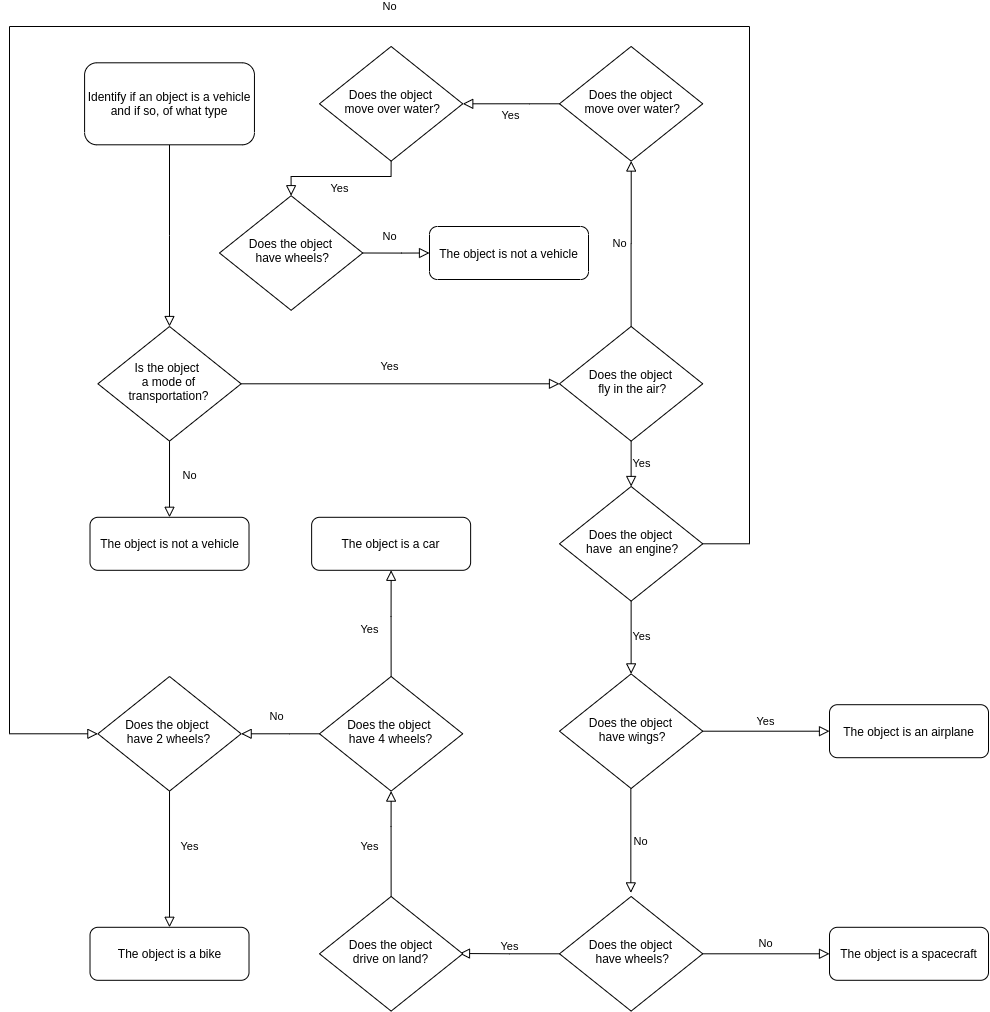
\includegraphics[width=\linewidth]{images/flowchart-prolog-vehicle-expert-system.png}
  \caption{This figure displays a decision tree that shows how our system could
  come to a conclusion in determining the type of a vehicle.}
  \label{fig:flowchart-expert-system}
\end{figure}


\section{Usage} \label{man-usage}
The application is run by providing the following command \textbf{isVehicle(X)}.
This will first check if we are looking to identify a vehicle.

If the user types `yes' the system agrees on a abstract data type `vehicle'.
This data type has multiple subtypes such as `land vehicle' or `air vehicle'.
At last we have the `unidentified vehicle'; this can be a car or boat.
The answer the system gives will be decided by the answers that the user provides.

\newpage
\section{Logic} \label{man-logic}
In this section we will provide an explanation of our code.
The code is included with comments to provide as reference for the explanation.

\begin{lstlisting}{}
% this will be the entry to our expert system
isVehicle(X) :- is_true('mode of transportation'), vehicle(X).

% the types of vehicle each type is part of an subtype
vehicle(airplane)  :- is_true('has wings'), air_vehicle().
vehicle(spaceCraft)  :- air_vehicle(), hasNoWheels().
vehicle(car)  :- is_true('has four wheels'), is_true('has enginge'), land_vehicle() .
vehicle(bike) :- is_true('has two wheels'), land_vehicle().
vehicle(cycle) :- is_true('has two wheels'), is_true('no engine'), land_vehicle().
vehicle(boat) :- is_true('has two wheels'), is_true('no engine'), boat_vehicle().

% the subtypes
land_vehicle() :-
	is_true('drives on land').
% check sub types
air_vehicle() :-
	is_true('fly in air'),
	is_true('has engine').

boat_vehicle() :-
	is_true("moves over water"),
    is_true("has no wheels").

hasNoWheels() :- not(is_true('has wheels')).

% helper method to generate questions
is_true(Q) :-
        format("~w?\n", [Q]),
        read(yes).
\end{lstlisting}

\newpage
\section{Queries} \label{man-queries}

\begin{figure}[!h]
    \centering
    \includegraphics[height=7cm]{images/weirdfout.png}
    \caption{Rare foutmelding}
    \label{fig:rareFout}
\end{figure}{}
